\section{Implementation of clockless AES}

The AES was written in Balsa in a way that support both Balsa and
Teak simulation and synthesis, avoiding incompatibilites. Focus was at
producing a correct implementation before performance and power, to
demonstrate the feasability of using the tools for relativly
large-scale implementations.

The AES was implemented in an architecture with four 128-bit
registers, two for the data, and two for the key and
key-expansion. Two registers is needed for each, as they are
implemented as single latches and not master/slave latches which does
not, by design, support auto assignments of the form 
$var := var + 1$. The architecture was designed with one control-input,
$instruction$ and two 32-bit data-ports; one for inputp and one for
output. Seven instructions was defined to load, permutate and unload
data from the 128-bit key AES-encryption-circuit.

\begin{description}
  \item[load\_data] Loads 4 32-bit words of data into $reg_0$.
  \item[load\_key128] Loads 4 32-bit words of key into $key_0$.
  \item[add\_key] Sets $reg_1 := reg_0 xor key_0$ and then sets $reg_0
    := reg_1$ and $key_1 := key_0$.
  \item[sub\_bytes] Calculates $reg_1 := SubBytes(ShiftRows(reg_0))$.
  \item[mix\_col\_expand] Calculates $reg_0 := MixColumns(reg_1)$, and
    $key_0 := ExpandKey(key_1)$.
  \item[skip\_mix\_expand] Only calculates $key_0 := ExpandKey(key_1)$.
  \item[output\_data] Outputs data in $reg_0$ as 4 32-bit words.
\end{description}


For the testbench, a module called aes\_ctrl issues instructions to
this module as follows:

\begin{figure}[htbp]
  \centering
  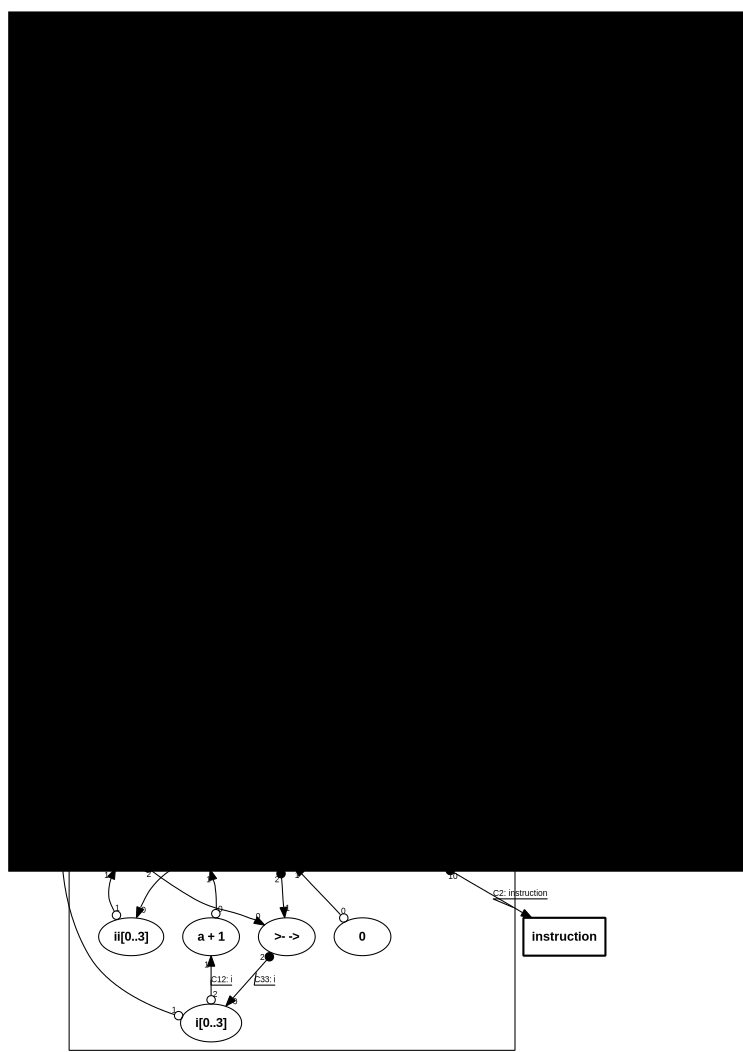
\includegraphics[height=0.9\textheight]{aesctrl.pdf}
  \caption{Source code for AES control module and Balsa handshake
    implementation}
  \label{fig:aesctrl}
\end{figure}


A 32 bit datapath was chosen for the same reasons given in
\cite{ekelund}, assuming that the same reasoning can be used for
clockless design.

The resources used in the top level design is:
\begin{itemize}
   \item 4 8-bit combinational SubBytes circuits, as as described in \cite{combsbox}, shared between the datapath and the keypath.
   \item 1 32-bit mixcolumn circuit
   \item 1 128-bit xor-adder circuit
\end{itemize}
